\documentclass{jsarticle}
\usepackage{moreverb}
\usepackage[dvipdfmx]{graphicx}
\usepackage{float}
\usepackage{amsmath}
\usepackage{amssymb}

\title{計算機実習 問題14.5 簡単な伝染病モデル}
\author{早稲田大学先進理工学部物理学科 B4 藤本將太郎}
\date{\today}

\begin{document}
\maketitle
    
    \section{シミュレーションの目的}
    自然界には,さまざまな場面でフラクタルな構造を持つものと出会うことがある.その一つの身近な例として,伝染病の簡単なモデルにおいて現れる性質について考えることにする.伝染病の広がりについて考えるとき,流行の条件を知りたいと思うのが普通である.伝染病の広がりの簡単な格子モデルをつぎのように定式化することができる.占有された格子点は病気に感染した人に対応する.初め,1つの感染した格子点があり,最隣接の4個の周辺の点(正方格子上で)に感染する可能性がある.つぎの分割時間で,それら4個の感染可能な格子点のそれぞれは確率$p$で占有される(感染する).もし感染可能な格子点が占有されなければ,その格子点は免疫があるとし,再び調べることはしない.つぎに,新しい感染可能な格子点を見出し,その病気の伝染が抑制されるか格子の境界に達するかまで続ける.この病気の広がりに関する成長モデルは,確率$p$のパーコレーション・クラスターと等価な,感染した格子点のクラスター形成することを確認せよ.唯一の違いはモデルに離散的な分割時間を導入したことである.問題14.5では,このモデルの性質のいくつかについて調べることにする.
    
    \section{作成したプログラム}
        本シミュレーションで作成したプログラムを以下に示す.
        
        \subsection{簡単な伝染病モデルを再現するプログラム}
            
            パーコレーション・クラスター1つを効率的に生成する1つの方法としてよく知られたアルゴリズムに,リースのアルゴリズムがある.これは次の手順を実行することと同等である.
            
            \begin{itemize}
                \item[1.] 種として格子点の1つが占有される.種の最隣接格子点(正方格子では4)を周辺の点と呼ぶ.
                \item[2.] 各周辺の点について,単位区間の乱数$r$を生成する.$r \le p$の場合にはその格子点は占有され,クラスターに加えられる.そうでない場合には占有されない.格子点が占有されない確率を$1-p$とするために,占有されなかった格子点について再び占有されるかどうか試すことはしない.
                \item[3.] 占有された各格子点について,新しい周囲の点,つまり試されていない隣接格子点が存在するかどうか調べる.周囲の点の表に新しい周辺の点を加える.
                \item[4.] 占有されるかどうかが試されていない周辺の点がなくなるまで,手順2と3を続ける.
            \end{itemize}

            このリースのアルゴリズムの一部を変更し,伝染病に関する簡単なシミュレーションを行う.確率$p$によって占有された(感染した)格子点は値1を持つとし,調べられたが占有されなかった格子点(免疫をもつ格子点)には値-1を代入していく.種を格子の中心の点とし,考えている格子の外側の領域はすべて-1の値を持たせておく.次にこのステップで占有された格子点に関して,その周囲でまだ試されていない格子点(値0を持つ)を探し,これを配列nnsiteに格納する.また,その格子点自身が系の端に位置するとき,集合lにその情報を記録しておき,端と端が連結したとき,この系はパーコレートしたとする.この過程を繰り返し,nnsiteに要素が含まれなくなったとき.または系がパーコレートしたときに過程を終了する(41〜67行目).関数perc\_clusterがこれらのアルゴリズムを実行する部分であり,各時刻$t$に関して,その時刻での周囲の点の数$S$と,占有された格子点の数$N$を記録している.関数を実行し終わった後には,これらの時系列でのデータが返され,関数内部で格子の占有状態が記録されている.以前に使用したdraw\_canvasやTopWindowクラス,plot\_graph関数を用いて,占有された格子点を描画したり,$S$,$N$についてのグラフを表示したりすることができるようにしてある.
            
            \listinginput{1}{14-5_infectious_disease_model.py}
            
            
    \section{実習課題}
    
        \begin{enumerate}
            \renewcommand{\labelenumi}{\alph{enumi}.}
            \renewcommand{\labelenumii}{}
            
            \item 感染可能な格子点が感染する確率を$p$とすると,本文で議論された簡単な伝染病のモデルが,リースのアルゴリズムと同じクラスターを生じる理由を説明せよ.広く伝染するために必要な$p$の最小の値はどれほどか.分割時間ごとに,すべての感染可能な格子点が同時に調べられ,確率$p$で感染することを忘れないこと.感染した格子点の数$N$がいろいろな$p$の値に対してどのように時刻$t$(分割時間の数)に依存するかを定めよ.これらを実行する直接的な方法は,プログラムperc\_clusterを修正して,新しい周辺の点を見出す前にすべての周辺の点を調べて確率$p$で占有されるようにすることである.第15章ではこのモデルがセルラーオートマトンの1つの例であることを学ぶ.
                
            \begin{enumerate}
                \item \ \ 2で示したようなアルゴリズムを用いたとき,このモデルはリースのアルゴリズムと同じクラスターを生じる.これは,この2つのモデルの間の相違というのが,離散的な時間間隔を導入しているかどうかの違いだけにある,ということに起因する.すなわち,リースのアルゴリズムにおいては格子の成長は一回にひとつずつであったが,伝染病モデルにおいては,分割時間ごとに,そのとき感染可能な格子点すべてに対して,占有するかどうかの操作が行われている.しかしながらこれは,調べられたが占有されなかった点を,まだ調べられていない格子点と区別していることによって,本質的な違いを生まない.実際,伝染病のモデルにおいても,結局は調べる格子1個1個に対して操作を順番に行っているのであり,複数の感染した格子点に囲まれていようが感染確率は$p$で変わらないことから,このアルゴリズムで生成された図形は,リースのアルゴリズムによって形成されたものと同じものであるということができる.
                
                \ \ 次に,感染した格子点の数$N$が時間$t$に対してどのように変動するかということを,さまざまな$p$の値に対して観察した.この結果を図\ref{fig:14-5-f1},\ref{fig:14-5-f2},\ref{fig:14-5-f3},\ref{fig:14-5-f4}(各上段)に示す.図から分かるように,どの$p$に対しても,$\ln N$はほぼ$\ln t$に比例しているように見える.また,$p=0.3$から$p=1.0$の間の$p$について,パーコレーション確率$P(p)$を試行回数200回のうち何回パーコレートしたかで求め,これを図\ref{fig:14-5-f5}に示す.図から,パーコレーション閾値$p_{c}$はおよそ$p=0.6$であることが分かる.これは,先ほどの考察で伝染病のモデルがリースのアルゴリズムと等価であることを示したが,このことから要求されるとおりに,通常のサイト・パーコレーションにおけるパーコレーション閾値と同じ値を持つことを表している.
                
                \begin{figure}[H]
                \begin{tabular}{cc}
                    \begin{minipage}{0.48\hsize}
                        \begin{center}
                            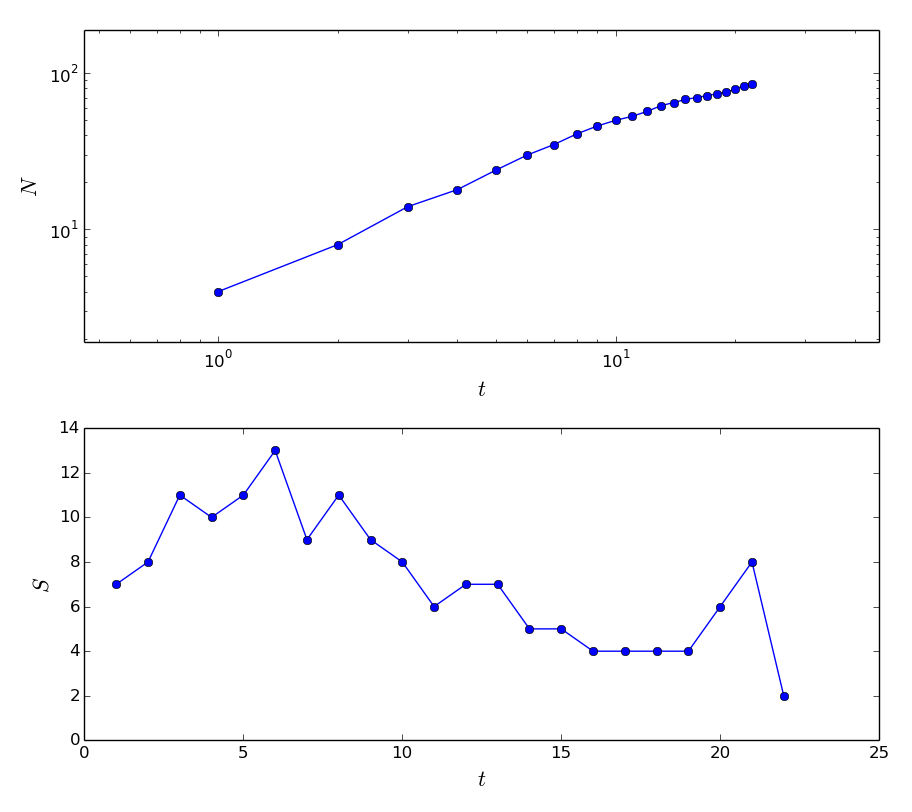
\includegraphics[width=6.0cm]{figure_1(p=05).png}
                            \caption{$p=0.5$のとき,時刻$t$と$N$,$S$の関係}
                            \label{fig:14-5-f1}
                        \end{center}
                    \end{minipage}
                    \begin{minipage}{0.48\hsize}
                        \begin{center}
                            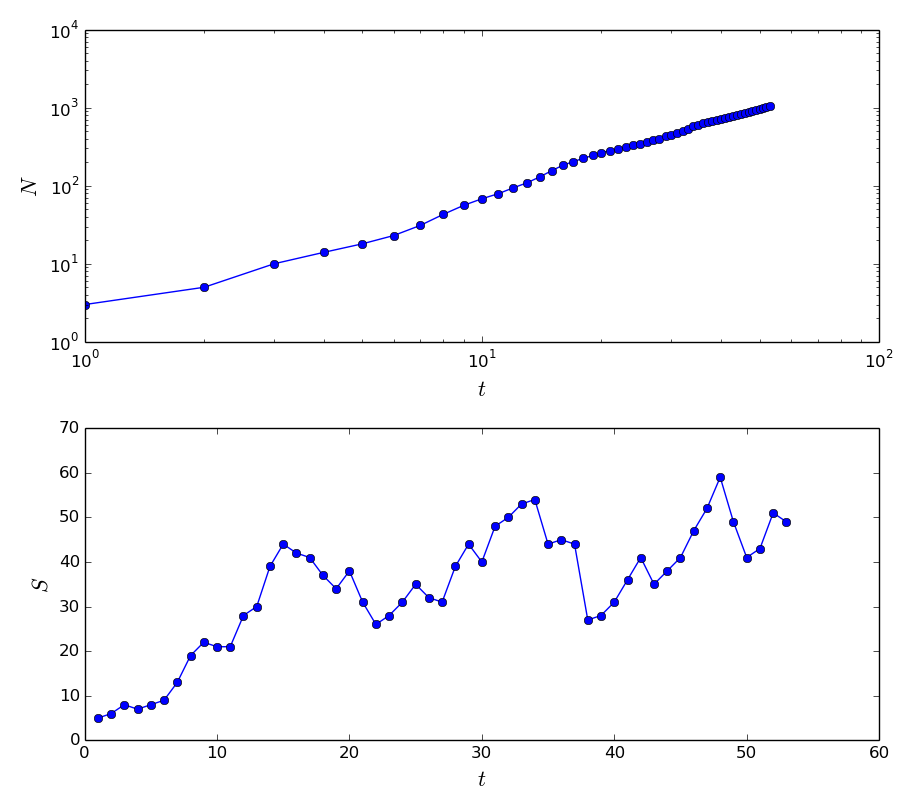
\includegraphics[width=6.0cm]{figure_1(p=06).png}
                            \caption{$p=0.6$のとき,時刻$t$と$N$,$S$の関係}
                            \label{fig:14-5-f2}
                        \end{center}
                    \end{minipage}\\
                    \begin{minipage}{0.48\hsize}
                        \begin{center}
                            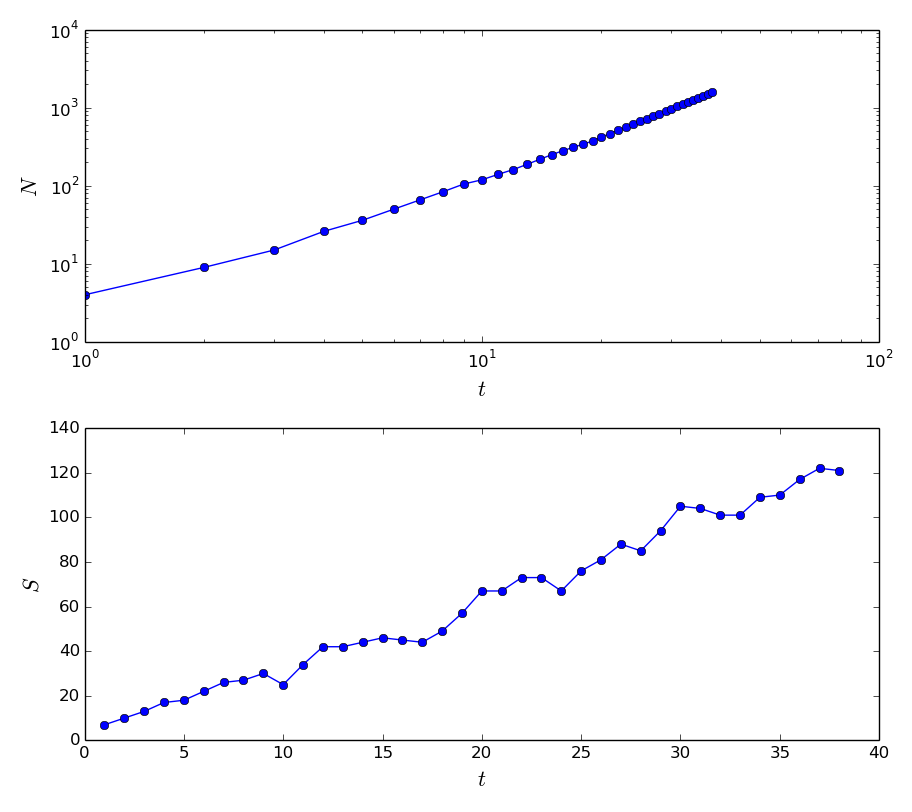
\includegraphics[width=6.0cm]{figure_1(p=07).png}
                            \caption{$p=0.7$のとき,時刻$t$と$N$,$S$の関係}
                            \label{fig:14-5-f3}
                        \end{center}
                    \end{minipage}
                    \begin{minipage}{0.48\hsize}
                        \begin{center}
                            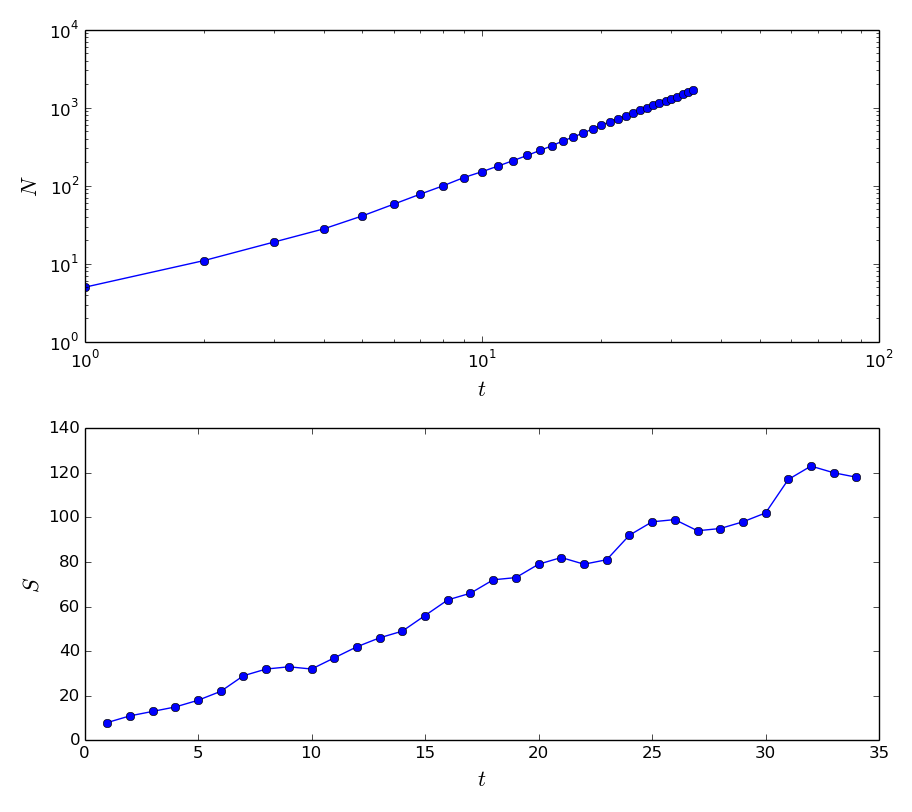
\includegraphics[width=6.0cm]{figure_1(p=08).png}
                            \caption{$p=0.8$のとき,時刻$t$と$N$,$S$の関係}
                            \label{fig:14-5-f4}
                        \end{center}
                    \end{minipage}
                \end{tabular}
            \end{figure}
                
            \begin{figure}[H]
                \begin{center}
                    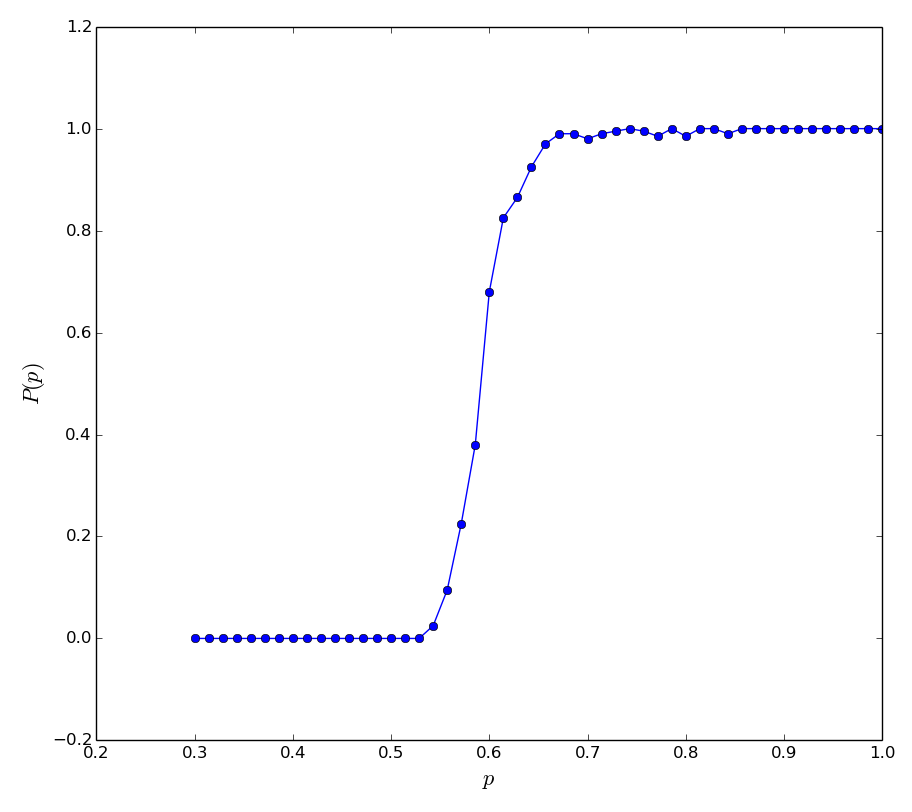
\includegraphics[width=9.0cm]{figure_4.png}
                    \caption{$p=0.3$から$p=1.0$までの$p$における,パーコレーション確率$P(p)$}
                    \label{fig:14-5-f5}
                \end{center}

            \end{figure}


            \end{enumerate}    
            
        \end{enumerate}
    
    \section{まとめ}
        
        簡単な伝染病のモデルについて,その性質のフラクタル性について考えることができた.
        
    \begin{thebibliography}{99}
        \bibitem{cite1}
        ハーベイ・ゴールド,ジャン・トボチニク,石川正勝・宮島佐介訳 『計算物理学入門』, ピアソン・エデュケーション, 2000.
        
    \end{thebibliography}     
\end{document}
